\newpage
\section{Character Kinematics}
运动学不涉及外来的力, 仅有角色自身的运动, 涉及外来力的专门叫物理仿真的方法. 

\subsection{Skeleton and forward Kinematics}

\subsubsection{Skeleton}

\begin{figure}[!htb]
    \centering
    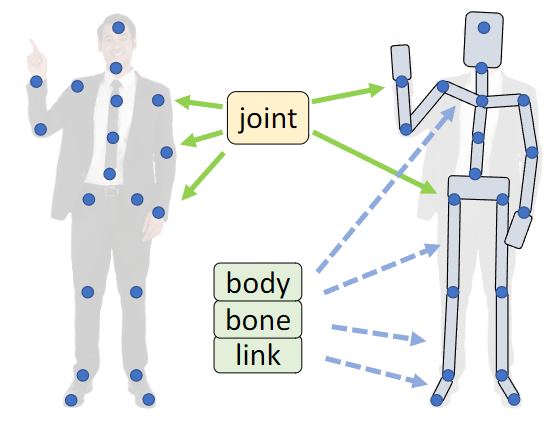
\includegraphics[width=0.618\linewidth]{pic/1053/Skeleton}
    \caption{Skeleton}
\end{figure}


\subsubsection{Kinematics of a Chain}

\begin{figure}[!htb]
    \centering
    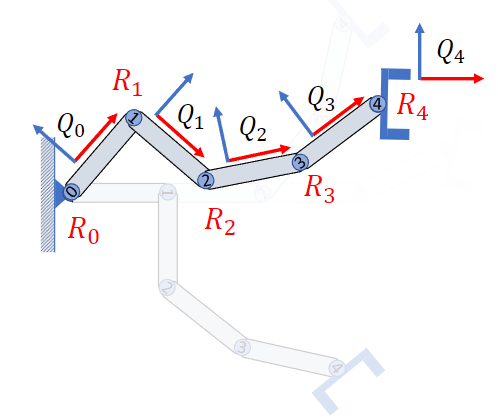
\includegraphics[width=0.618\linewidth]{pic/1053/Kinematics of a Chain}
    \caption{Kinematics of a Chain}
\end{figure}

\begin{itemize}
    \item $Q_i$: orientation of joint $i$.  (相对于全局的方向)
    \item $R_i$: rotation of joint $i$. (相对于上一个关节的旋转)
    \item $\bp_i$: positon. 全局坐标系下到 $i$ 的位置向量
    \item $\bl_i$: offset, translation. 从 $i$ 到 $i+1$ 的局部坐标系位置向量, 固定的. 即使所有的 $R_i$ 都为 $I$, $\bl_i$ 也可以构成一个动作, 这就是参考动作, 所有的关节旋转都是基于参考动作之上的. 
\end{itemize}

From rotation to orientation:
\begin{align*}
    Q_i=Q_{i-1}R_i
\end{align*}

From orientation to rotation
\begin{align*}
    R_i=Q_{i-1}^\top Q_i
\end{align*}

Relative rotation:
\begin{align*}
    R_4^1&=Q_1^\top Q_4\\
    &= (R_0R_1)^\top R_0 R_1 R_2R_3R_4\\
    &=R_2R_3R_4
\end{align*}
这是将局部坐标系变化为全局坐标系.
\begin{align*}
    \bp_i=\bp_{i-1}+Q_{i-1}\bl_{i-1}
\end{align*}

\begin{figure}[!htb]
    \centering
    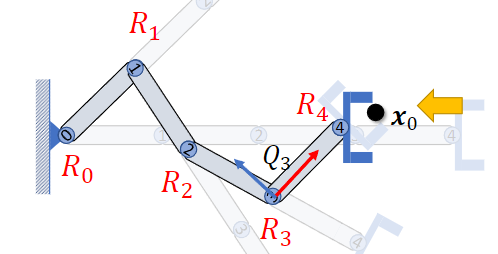
\includegraphics[width=0.618\linewidth]{pic/1053/反向求解}
    \caption{坐标系变换}
\end{figure}
这里 $\bx_0$ 在 4 的坐标系下, $\bx$ 在全局坐标系下, 若要求在 3 的坐标系下的 $\bx^{Q_3}$
\begin{align*}
    \bm x&=\bp_4+Q_4\bx_0\\
    &=\bp_3+Q_3(\bl_3+R_4\bx_0)\\
    \bx^{Q_3}&=Q_3^\top(\bx-\bp_3)\\
    &=\bl_3+R_4\bx_0
\end{align*}


\subsubsection{Kinematics of a Character}

\begin{figure}[!htb]
    \centering
    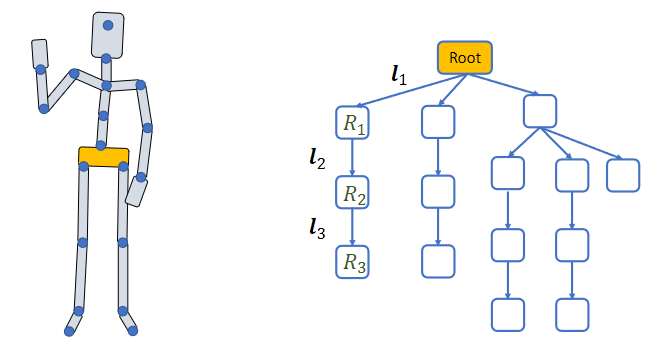
\includegraphics[width=0.618\linewidth]{pic/1053/Kinematics of a Character}
    \caption{Kinematics of a Character}
\end{figure}



\begin{definition}[Degrees of Freedom (DoF)]
    Number of independent parameters that define the configuration or state of
a mechanical system. 
\end{definition}

Types of Joints:
\begin{figure}[!htb]
    \centering
    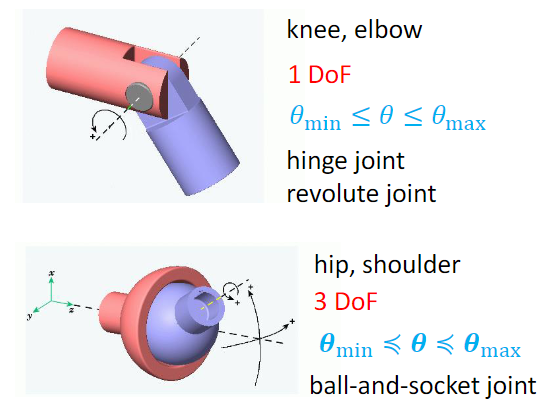
\includegraphics[width=0.618\linewidth]{pic/1053/Types of Joints}
    \caption{Types of Joints}
\end{figure}

Pose Parameters: 
\begin{align*}
    (\bt_0, R_0, R_1,R_2,\dots)
\end{align*}
where $\bt_0$ is root, $R_i$ is internal joints.



\subsection{Inverse Kinematics}

\subsubsection{Forward and Inverse Problems}

\subsubsection{Inverse Kinematics}
Given the position of the end-effector $\bx_i$, compute the joint rotations $R_i$, rotation parameters $\bm{\theta}_i$.


\begin{figure}[!htb]
    \centering
    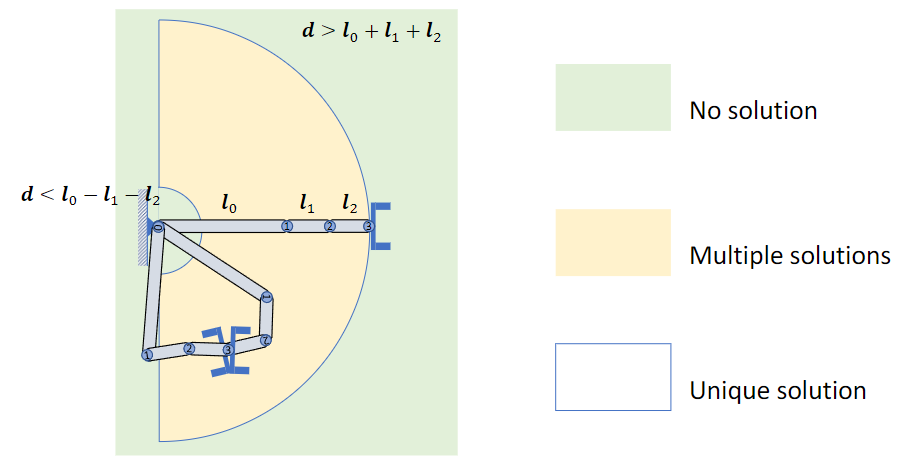
\includegraphics[width=0.618\linewidth]{pic/1053/Solutions of IK Problems}
    \caption{Solutions of IK Problems}
\end{figure}


\begin{example}
    Two-Joint IK
    \begin{figure}[!htb]
        \centering
        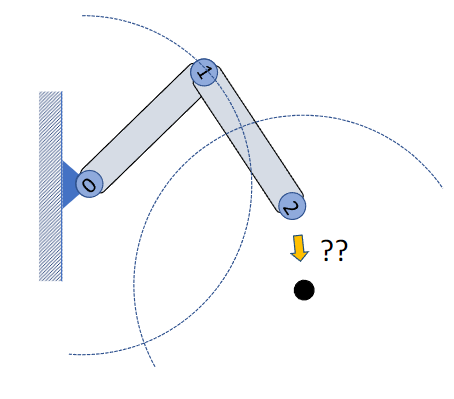
\includegraphics[width=0.618\linewidth]{pic/1053/Two-Joint IK}
        \caption{Two-Joint IK}
    \end{figure}
    
    \begin{enumerate}
        \item Rotate joint 1 such that
        \begin{align*}
            \norm{\bl_{0x}}=\norm{\bl_{02}}
        \end{align*}
        \item Rotate joint 0 such that
        \begin{align*}
            \bl_{0x}=\bl_{02}
        \end{align*}
        \item Rotate joint 0 around $\bl_{0x}$ if necessary.
    \end{enumerate}

\end{example}

\subsubsection{IK as an Optimization Problem}
For an IK problem, find $\bm\theta$ to optimize
\begin{align*}
    \min_{\btheta} &F(\btheta)\\
    F(\theta)&=\frac{1}{2}\norm{f(\btheta)-\tilde{\bx}}_2^2
\end{align*}
这里 $\frac{1}{2}$ 是为了求导方便. 

\subsubsection{Cyclic Coordinate Descent (CCD) IK}
Iteratively rotation each joint to make the end-effector align with vector between the joint and the target.

Easy to implement, very fast. Result can be sensitive to the initial solution.

相当于每次对一个参数求解一个优化问题, 迭代所有参数, 直到收敛.

\subsubsection{Gradient Descent}
求 
\begin{align*}
    \bx=f(\theta_0,\theta_1,\dots)
\end{align*}
的梯度, 进行下降. 

\begin{itemize}
    \item Finite Differencing
    \item Geometric Approach
\end{itemize}



Update parameters against the direction of the gradient of the objective function
\begin{align*}
    \btheta^{i+1}&=\btheta^i-\alpha \nabla_\btheta F(\btheta^i)
\end{align*}
\begin{itemize}
    \item Jacobian Transpose Method
    \begin{align*}
        \btheta=\btheta^i-\alpha J^\top \Delta
    \end{align*}
    \item Jacobian Inverse Method (因为 $J$ 做不了逆, 所以做伪逆 $J^+$)
    \begin{align*}
        \btheta^{i+1}=\btheta^i-\alpha J^+ \Delta
    \end{align*}
\end{itemize}

First-order approach, convergence can be slow. Need to re-compute Jacobian at each iteration.

对于 $J$ 的计算, 要么用 pytorch 自动计算, 要么就是手算. 

\subsubsection{Gauss-Newton Method}

\subsubsection{Jacobian Inverse Method}

\subsubsection{Damped Jacobian Inverse Method}
Using the minimal rotations to reach the target

\subsubsection{Character IK}

\begin{figure}[!htb]
    \centering
    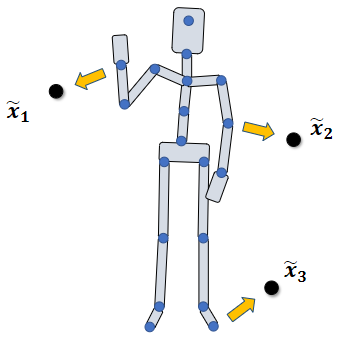
\includegraphics[width=0.42\linewidth]{pic/1053/Character IK}
    \caption{Character IK}
\end{figure}

\begin{align*}
    F(\theta)&=\frac{1}{2}\sum_i \norm{f_i(\btheta)-\tilde{\bx}_i}_2^2+\frac{\lambda}{2}\norm{\btheta}_2^2\\
    \btheta&=(\bt_0, R_0, R_1, R_2,\dots)
\end{align*}
Consider one constraint each time, then fix the broken one. 

Character Rig: Created Multiple IK chains. User activates several IK chains each time, the joints controlled by the other IK chains can move freely.


\subsection{Posed Character}
会有很多种初始的 pose. 一般动捕用的是 t-pose, 但是做绑定的可能更喜欢 a-pose, 甚至某种奇怪的 pose. 


\subsection{Motion Retargeting}
同样的运动在不同的参考运动下会有不同的结果. 因为运动是用局部旋转描述的, 参考运动不同, 旋转的最终结果就不同. 

动作重定向甚至还有其他问题, 比如说关键长度, 或者穿模, 但目前不讨论. 

\subsubsection{Retargeting between reference poses}
在不同参考运行之间进行重定向. 

\begin{figure}[!htb]
    \centering
    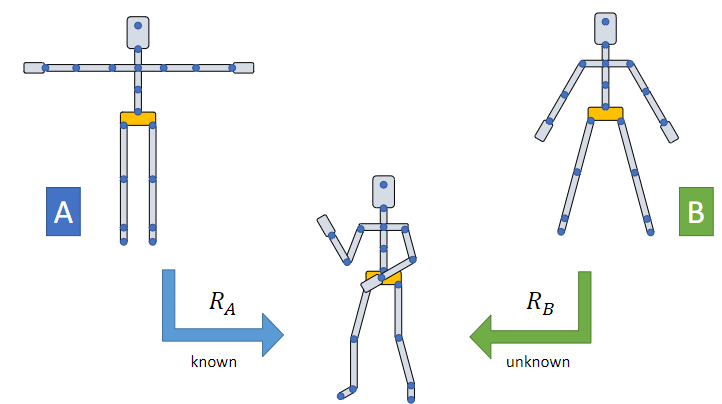
\includegraphics[width=0.618\linewidth]{pic/1053/Retargeting between reference poses}
    \caption{Retargeting between reference poses}
\end{figure}

\begin{figure}[!htb]
    \centering
    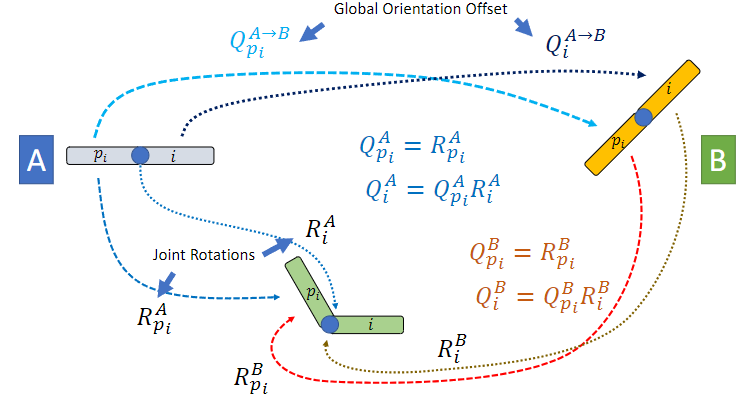
\includegraphics[width=0.88\linewidth]{pic/1053/Retargeting for a chain of links}
    \caption{Retargeting for a chain of links}
\end{figure}

$p_i$ 代表 $i$ 的 parent.
\begin{align*}
    Q^B&=Q^A(Q^{A\to B})^\top\\ 
    R_i^B &= (Q_{p_i}^B)^\top Q_i^B \\
    &= Q_{p_i}^{A\to B}(Q_{p_i}^A)^\top Q_i^A (Q_i^{A\to B})^\top \\
    &= Q_{p_i}^{A\to B}R_i^A(Q_i^{A\to B})^\top
\end{align*}



